\documentclass{beamer}

\usepackage[utf8]{inputenc}
\usepackage{tikz}
\usepackage{gnuplottex} % [noshell]: do not regenerate gnuplots
\usepackage{booktabs}
\usepackage{listings}
\lstset{
  language=python,
  basicstyle=\scriptsize,
}
\usetheme{ODK}

\AtBeginSection[]
{
  \begin{frame}<beamer>
    \frametitle{Outline}
    \tableofcontents[currentsection]
  \end{frame}
}

\title[Workpackage 5]{Workpackage 5:\\ High Performance Mathematical Computing}

\author[2nd projet review]{Clément Pernet}

\date{Luxembourg, October 30, 2018}

\institute[ODK Project review]{Second OpenDreamKit Project review}

\begin{document}
\maketitle

%%%%%%%%%%%%%%%%%%%%%%%%%%%%%%%%%%%%%%%
\section*{Introduction}

\begin{frame}
  \frametitle{High performance mathematical computing}

  \begin{block}{Computer algebra}
    Typical computation domains:
    \begin{itemize}
    \item $\mathbb{Z}, \mathbb{Q}$: $\leadsto$ multiprecision integers
    \item $\mathbb{Z}/p\mathbb{Z}, \mathbb{F}_q$: $\leadsto$ machine ints or
      floating point, multiprecision
    \item $K[X], K^{m\times n}$, $K[X]^{m\times n}$ for $K=\mathbb{Z},\mathbb{Q},\mathbb{Z}/p\mathbb{Z}$
    \end{itemize}
  \end{block}

  \begin{block} {High performance computing}
    \begin{itemize}
    \item Decades of development for numerical computations
    \item Still at an early development stage for computer algebra
    \item Specificites: cannot blindly benefit from numerical HPC experience
    \end{itemize}
  \end{block}
\end{frame}
%%%%%%%%%%%%%%%%%%%%%%%%%%%%%%%%%%%%%%%%%%%%%%%%%%%%%%%%%%%%%%%%%
\begin{frame}
  \frametitle{Goal: delivering high performance to maths users}

\uncover<2->{
  \only<1,2>{
    \begin{block}{Harnessing modern hardware $\leadsto$ parallelisation}
  \begin{itemize}
    \item in-core parallelism (SIMD vectorisation)
    \item multi-core parallelism
    \item distributed computing: clusters, cloud
    \end{itemize}
  \end{block}
  }
  
  \only<3>{
    \begin{block}{Languages}
    \begin{itemize}
    \item Computational Maths software uses high level languages (e.g. Python)
    \item High performance delivered by languages close to the metal (C, assembly)
    \end{itemize}
    $\leadsto$ compilation,  automated optimisation
  \end{block}
  }
  }
  \begin{center}
    \only<1>{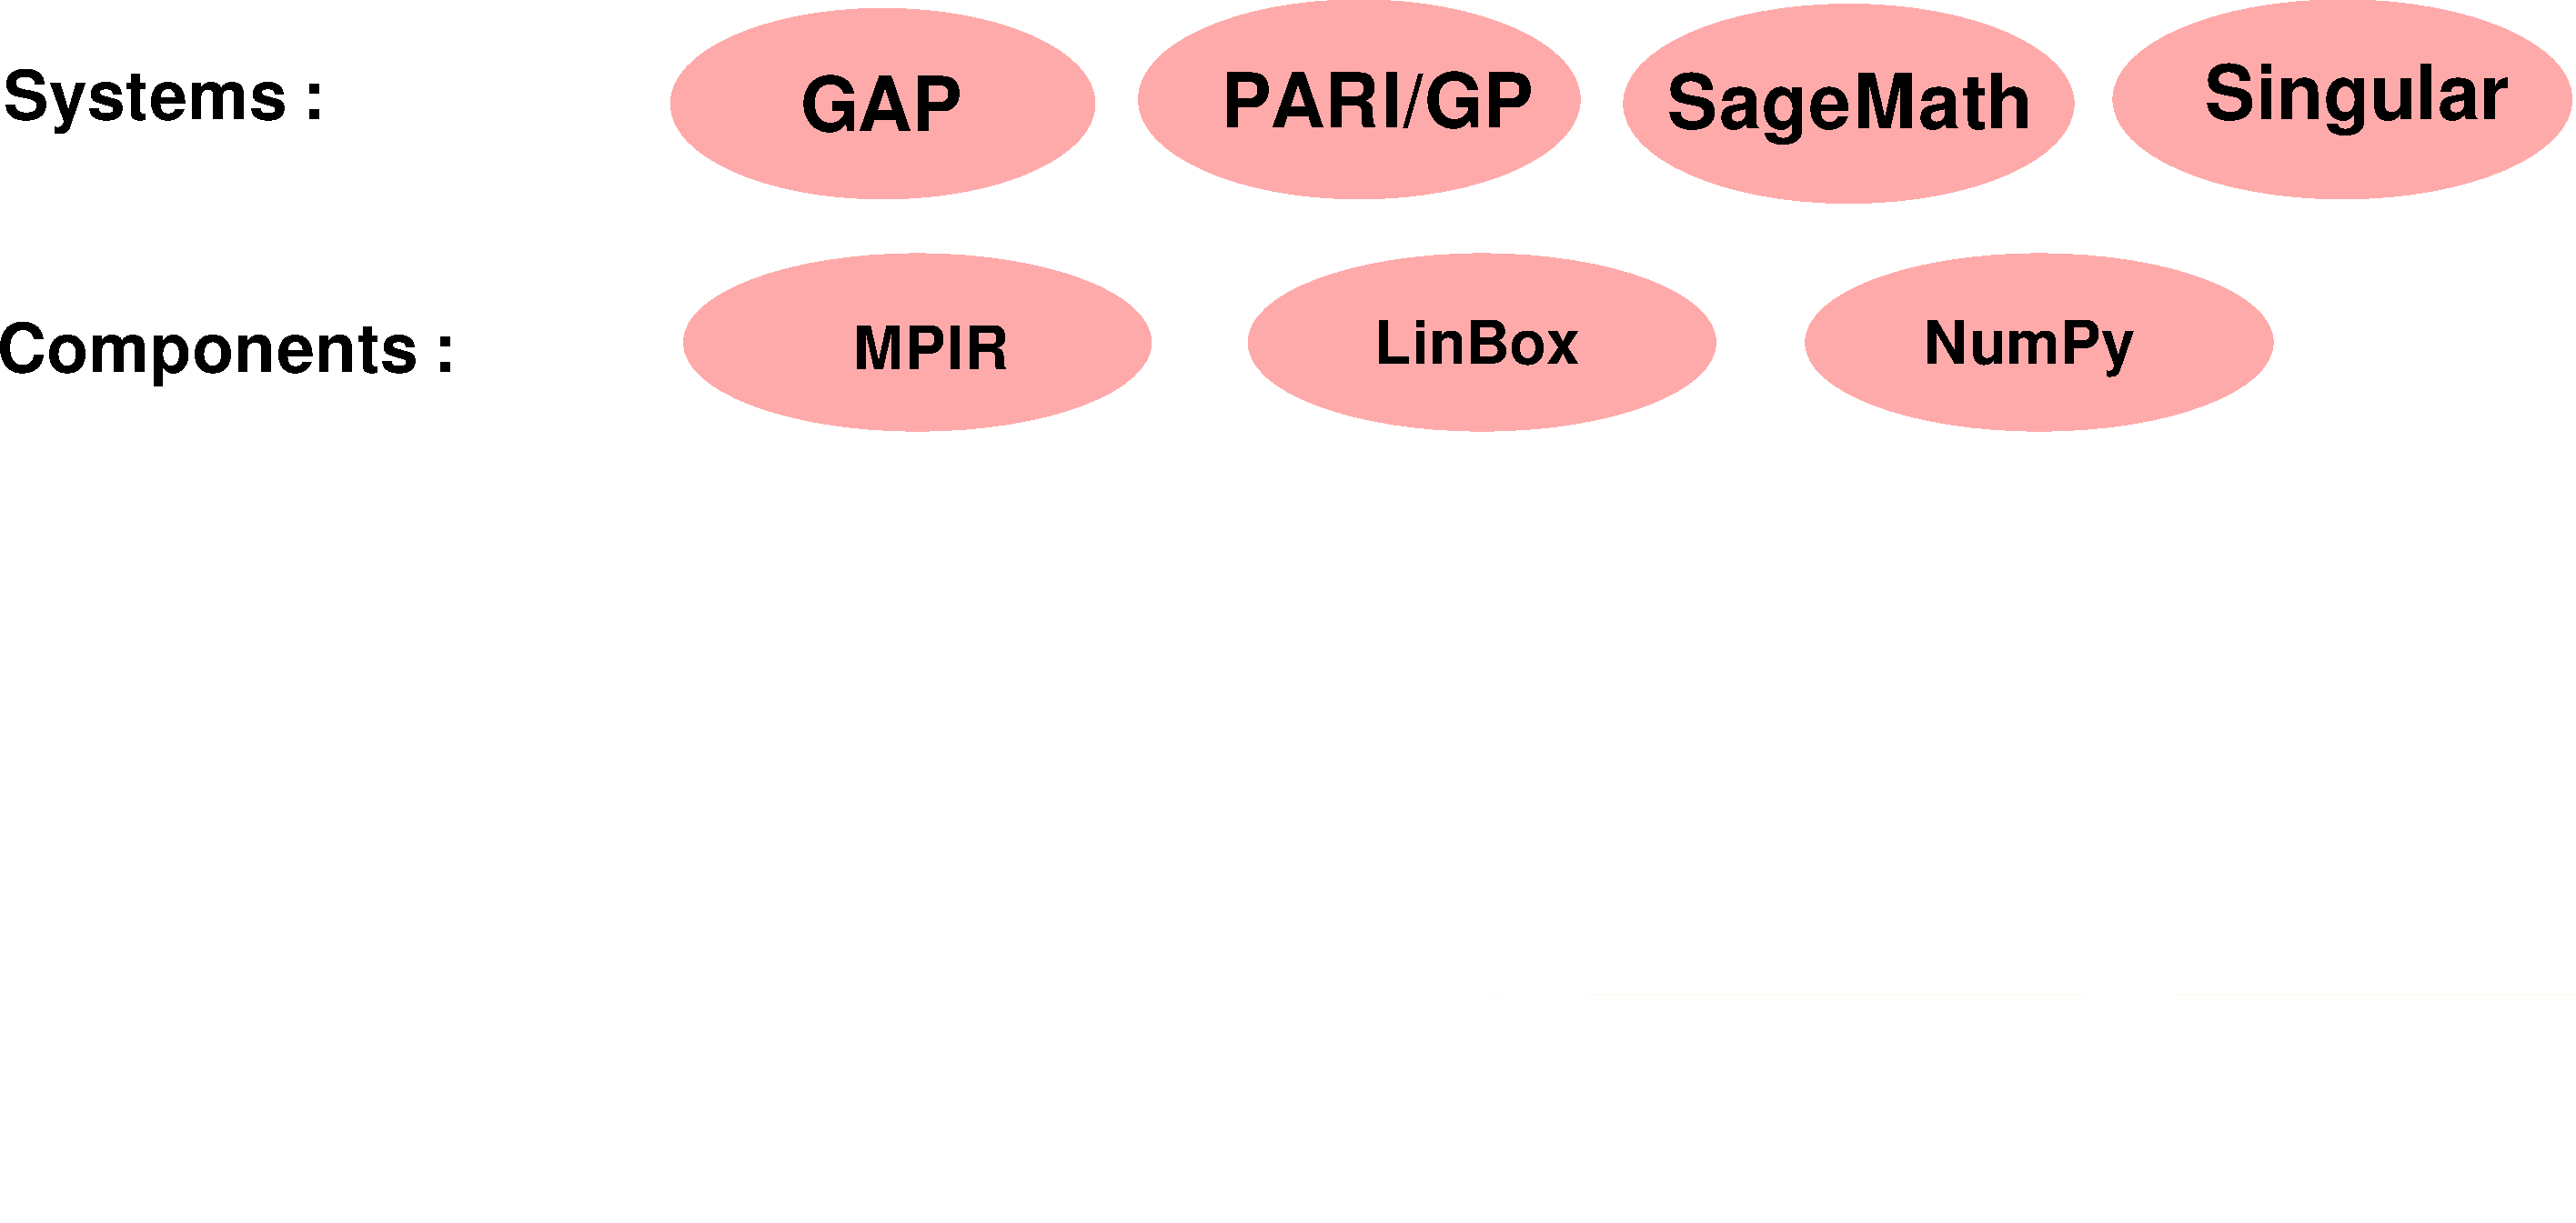
\includegraphics[width=0.8\textwidth]{software_stack_3}}

    \only<2>{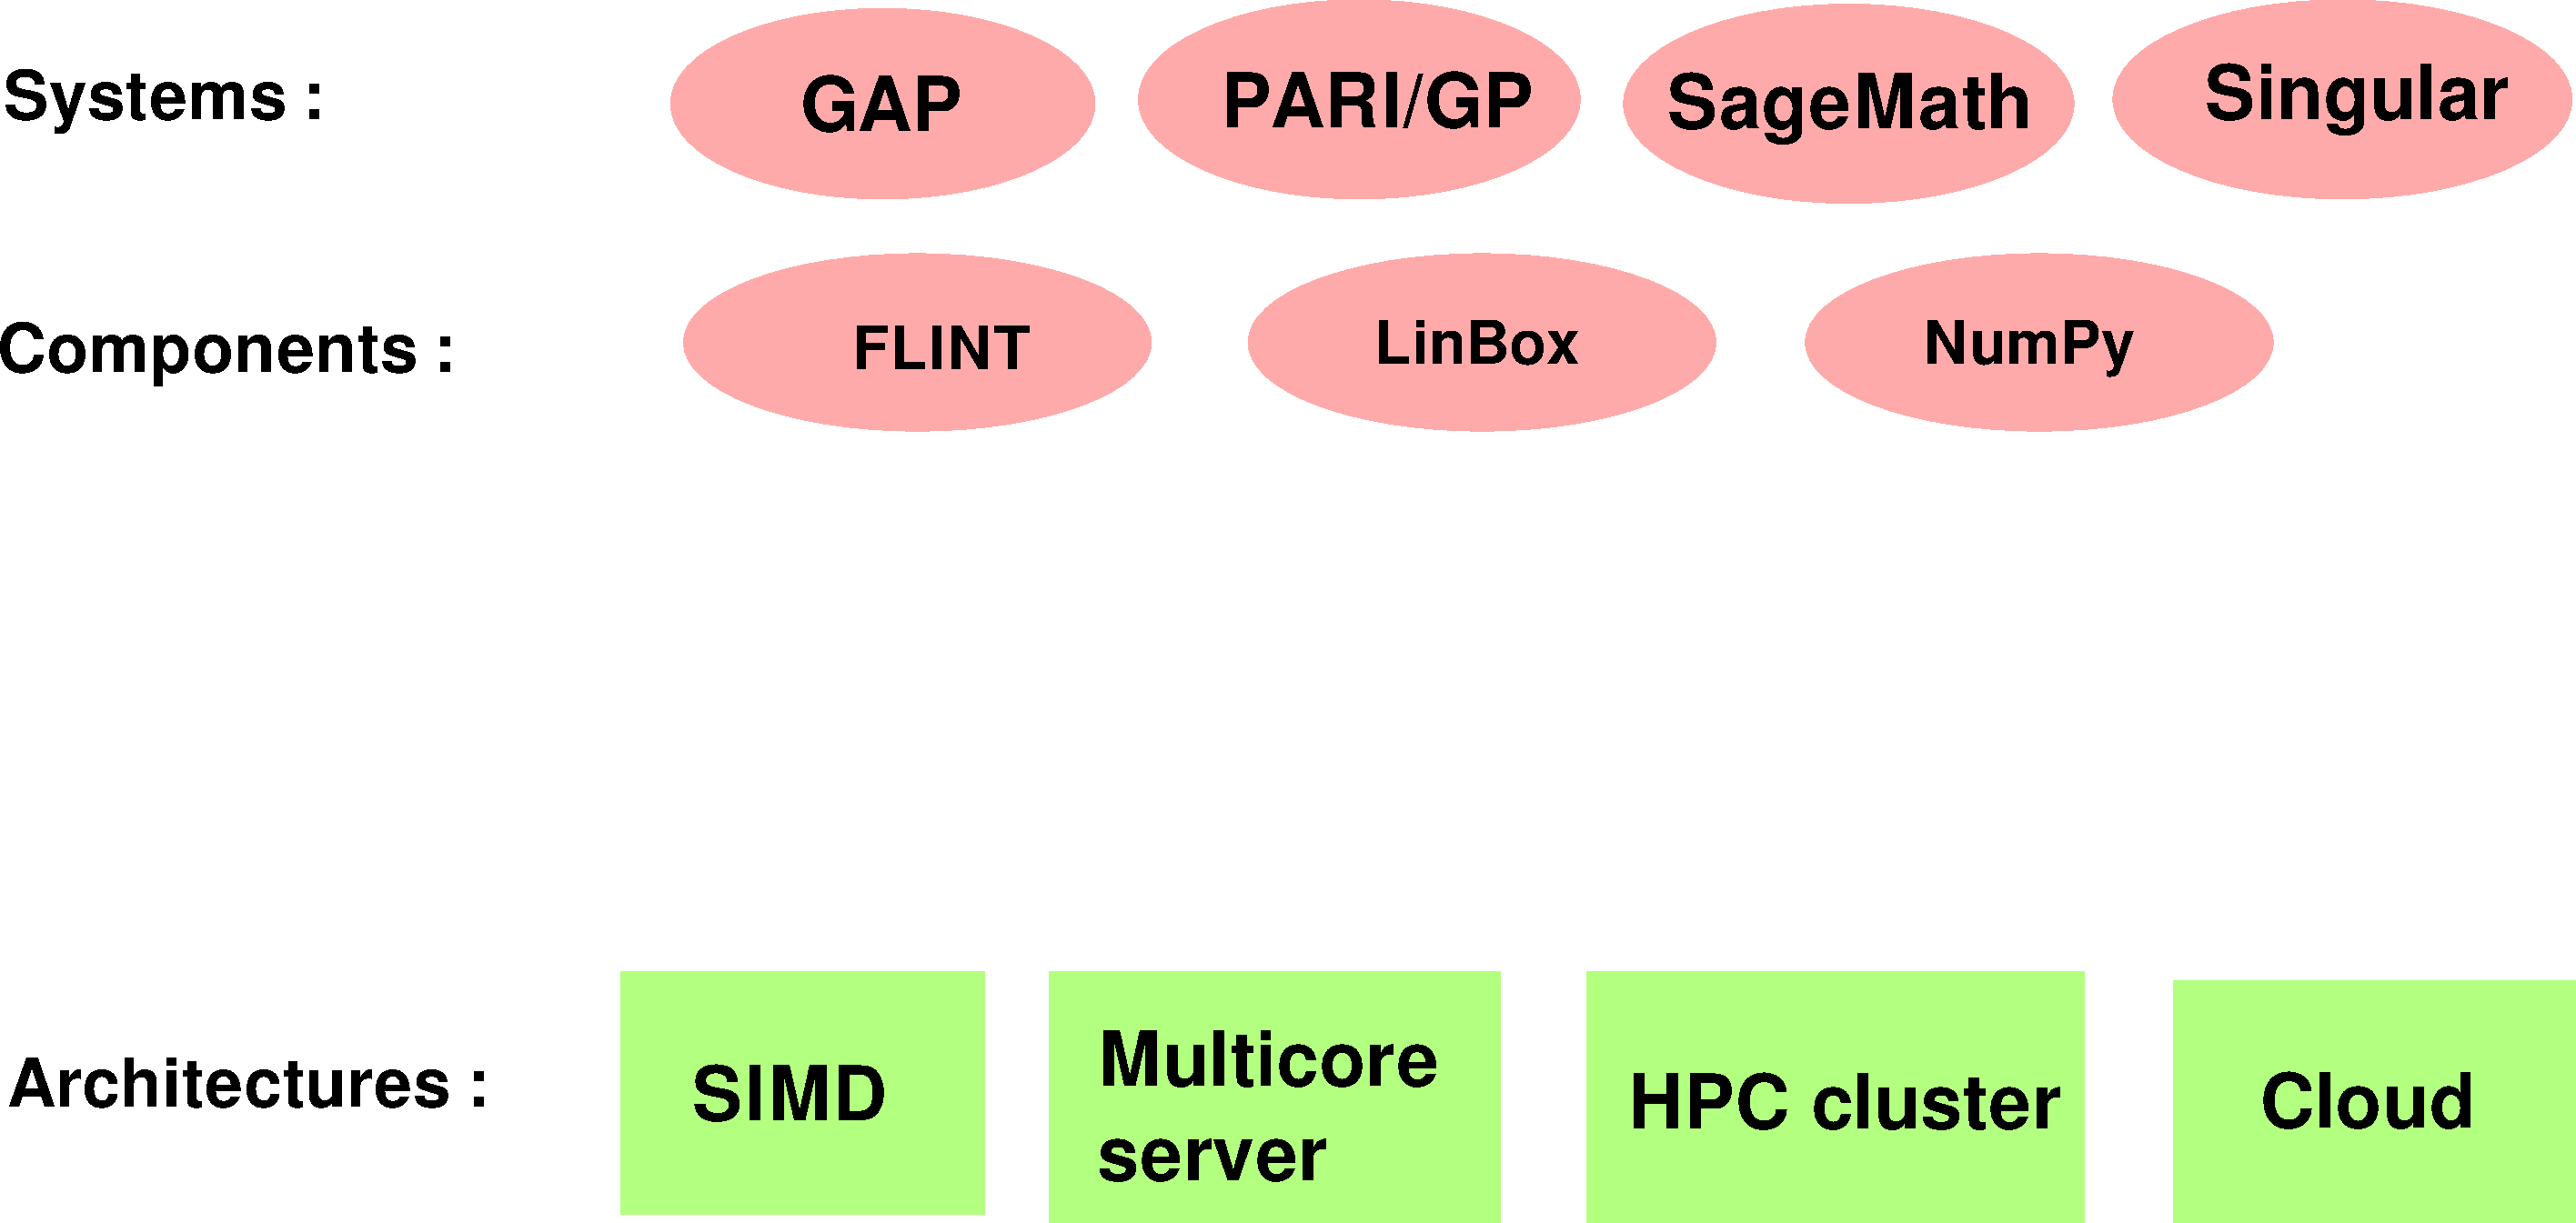
\includegraphics[width=0.8\textwidth]{software_stack_2}}
    
    \only<3>{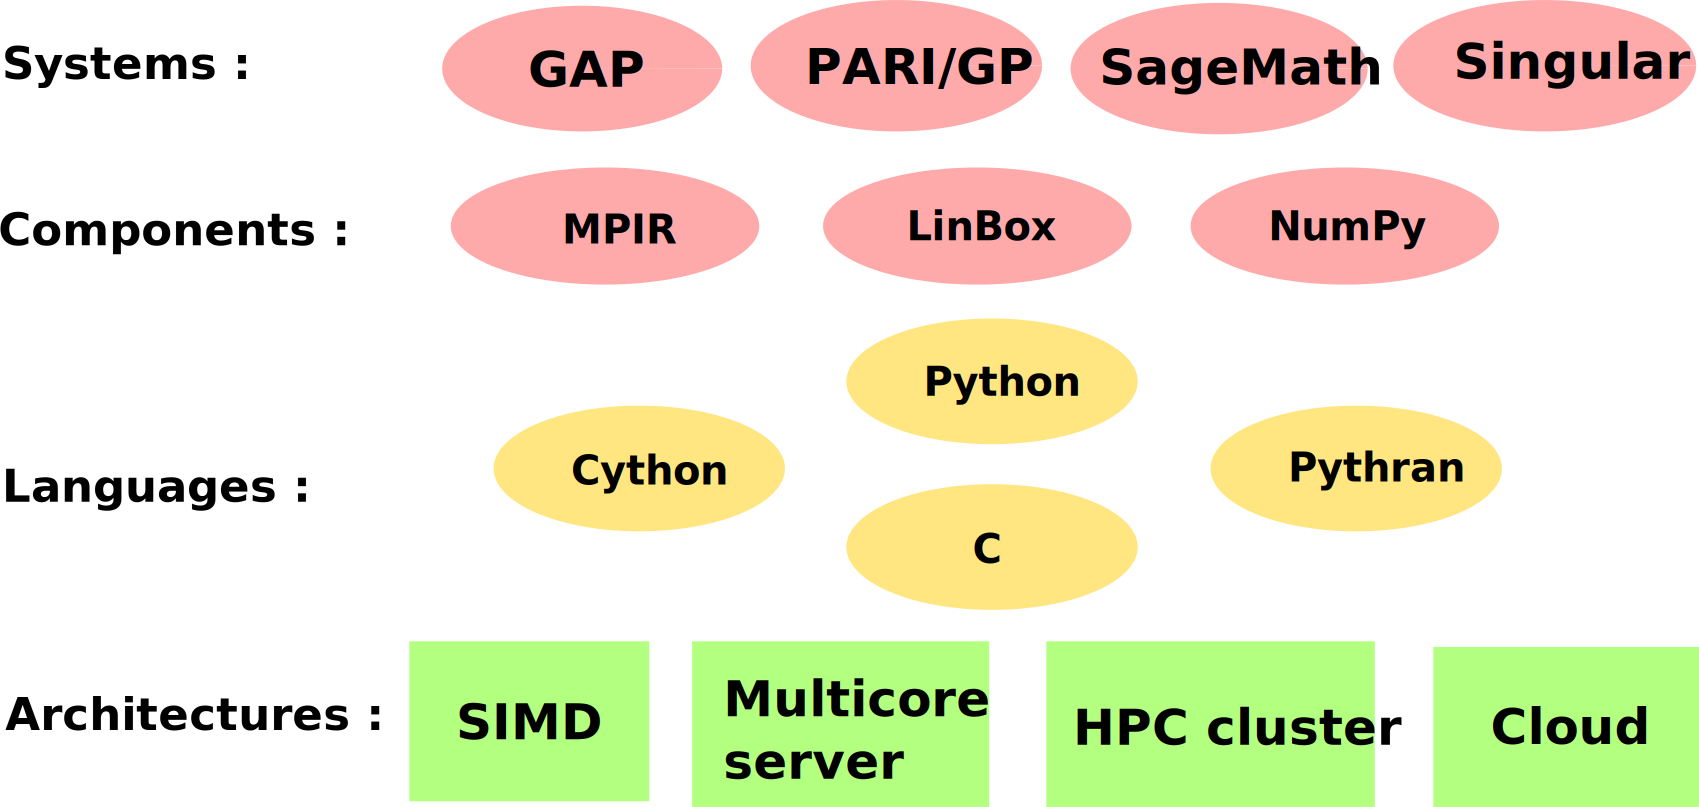
\includegraphics[width=0.8\textwidth]{software_stack}}
\end{center}

\end{frame}
%%%%%%%%%%%%%%%%%%%%%%%%%%%%%%%%%%%%%%%%%%%%%%%%%%%%%%%%%
%% \begin{frame}
%%   \frametitle{Goal: delivering high performance to maths users}

%%     \begin{center}
%%     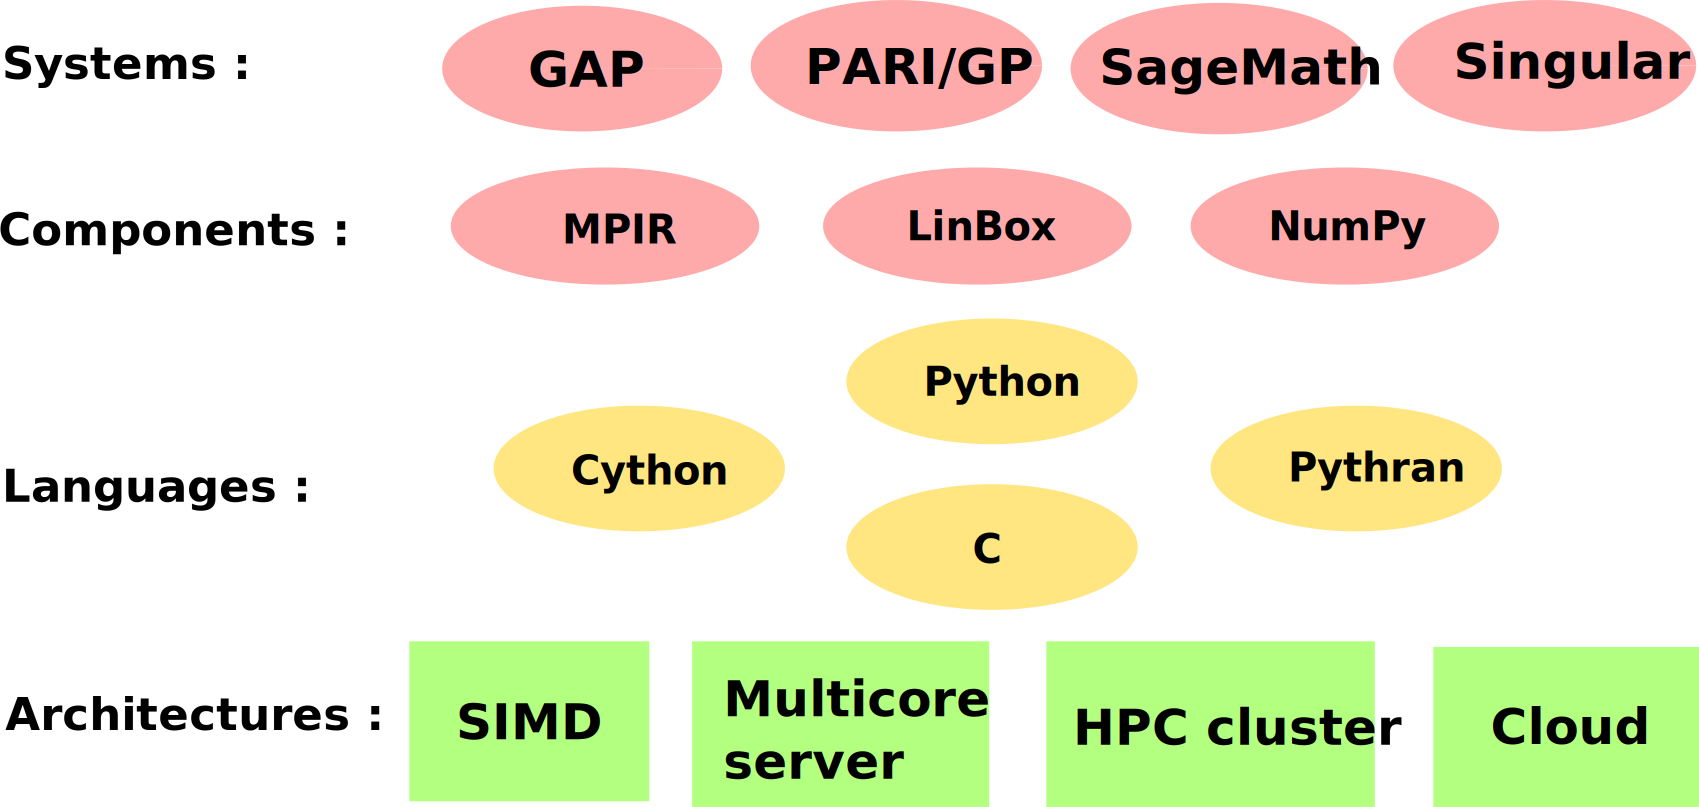
\includegraphics[width=0.8\textwidth]{software_stack}
%%   \end{center}

%%     \pause
%%     \begin{itemize}
%%     \item Improve/Develop parallel features of components first,
%%     \item Expose them through the software stack
%%     \item 
%%     \end{itemize}

%% \end{frame}


%%%%%%%%%%%%%%%%%%%%%%%%%%%%%%%%%%%%%%%
\begin{frame}
  \frametitle{Introduction}
  \begin{block}
    {Goal:}
    \begin{itemize}
    \item Improve/Develop parallel computing features of dedicated software
      kernels
    \item Expose them through the software stack
    \item Offer High Performance Computing to VRE's users
    \end{itemize}
  \end{block}
\end{frame}
%%%%%%%%%%%%%%%%%%%%%%%%%%%%%%%%%%%%%%%%%%%%%%%%%%%%%%
\begin{frame}
\frametitle{Addressing recommendations of review 1}
    \textbf{Recommendation 10:} \textit{Regarding WP5, \textbf{make contacts} with HPC community in order to ascertain current state-of-the-art. The work in this WP needs to be \textbf{nearer the leading edge}.}

    \begin{description}
    \item<2-> [Leading edge achievements in linear algebra] \
      {\small
      \begin{itemize}
      \item symmetric factorization outperforms LAPACK implementation
      \item new non-hierarchical generator for quasiseparable matrices
      \item large scale parallelization of rational linear solver
      \end{itemize}
      }
    \begin{columns}
      \begin{column} {.3\textwidth}
        \begin{center}
          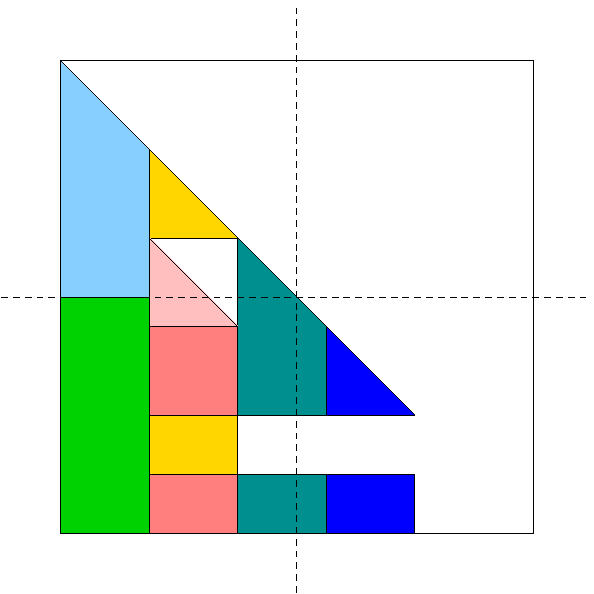
\includegraphics[width=.6\textwidth]{ARrec11}
      \end{center}
      \end{column}
      \begin{column} {.3\textwidth}
        \begin{center}
          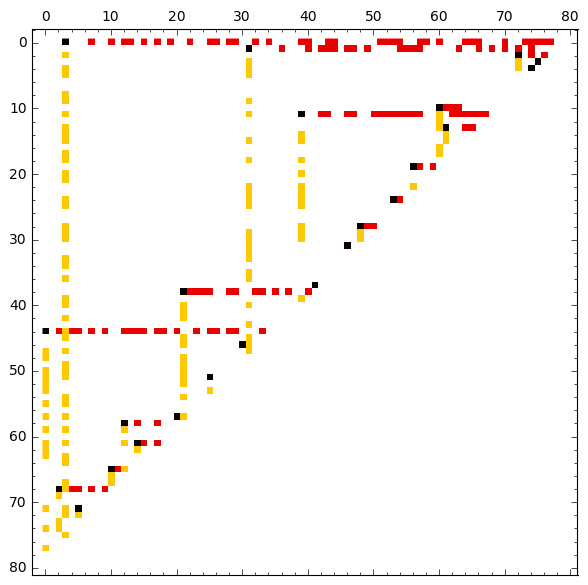
\includegraphics[width=.6\textwidth]{Bruhat}
        \end{center}
      \end{column}
      \begin{column} {.3\textwidth}
        \begin{center}
          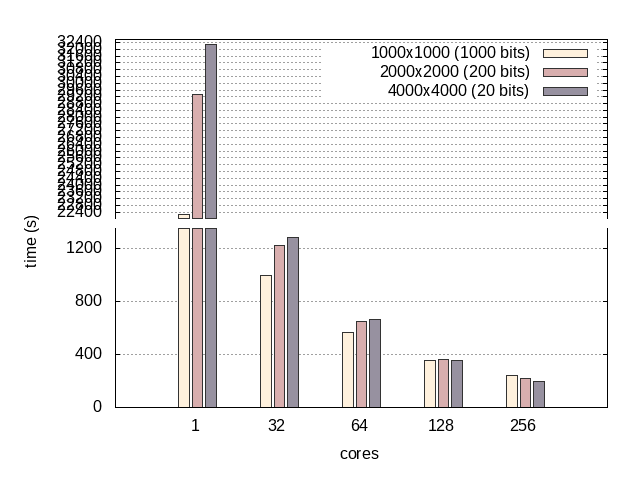
\includegraphics[width=.9\textwidth]{nodes_histogram}
        \end{center}
      \end{column}
    \end{columns}
    \item<3-> [Interactions and  contacts made:]\ 
      {\small
      \begin{itemize}
      \item interaction with the \texttt{BLIS} group (vectorization and
        implementation of Strassen's algorithm)
      \item on-going collaboration with T. Mary (\texttt{Mumps}) and
        S. Chandrasekaran (UCSB) on quasiseparable matrix algorithmic
      \end{itemize}
      }
\end{description}
\end{frame}

%%%%%%%%%%%%%%%%%%%%%%%%%%%%%%%%%%%%%%%
\begin{frame}
  {Outline}
  \tableofcontents
\end{frame}

%%%%%%%%%%%%%%%%%%%%%%%%%%%%%%%%%%%%%%%
\section{Deliverables under review for the period}
%%%%%%%%%%%%%%%%%%%%%%%%%%%%%%%%%%%%%%%
\subsection{D5.12: Exact linear algebra algorithms and implementations.}

\begin{frame}
  \frametitle{Task 5.3: LinBox, High performance exact linear algebra}

  \begin{block} {Linear algebra: a HPC building block}
    Similarly as in numercial HPC:
    \begin{itemize}
    \item central elementary problem to which others reduce to
    \item (rather) simple algorithmic
    \item high compute/memory intensity
    \end{itemize}
  \end{block}
    \begin{block}{Specificities}
      \begin{itemize}
      \item Multiprecision arithemtic $\Rightarrow$ lifting from finite  precision ($\mathbb{F}_p$)
      \item Rank deficiency $\Rightarrow$ unbalanced dynamic blocking
      \item Early adopter of subcubic matrix arithemtic $\Rightarrow$ recursion
      \end{itemize}
    \end{block}
      
    \end{frame}
%%%%%%%%%%%%%%%%%%%%%%%%%%%%%%%%%%%%%%%%%%%%%%%ù
\begin{frame}
  \frametitle{D5.12: Exact linear algebra algorithms and implementations. Library maintenance and close integration in mathematical software for LinBox library}

  \begin{enumerate}
  \item Algorithmic innovations:
    \begin{enumerate}
    \item Rank deficient dense Gaussian elimination
    \item Quasiseparable matrices
    \item Outsourced computing security
    \end{enumerate}
  \item Software releases and integration:
    \begin{enumerate}
    \item LinBox ecosystem: \texttt{LinBox, fflas-ffpack, givaro}
    \item \texttt{SageMath} integration
    \end{enumerate}
  \end{enumerate}
\end{frame}

%%%%%%%%%%%%%%%%%%%%%%%%%%%%%%%%%%%%%%%
\begin{frame}
  \frametitle{Rank deficient dense Gaussian elimination}
  \begin{block}
    {[JSC'17] Fast computation of the rank profile matrix and the generalized
      bruhat decomposition.}
{    \small
  \begin{itemize}
    \item Connecting Rank Profile Matrix and row and column echelon forms
    \item $O\tilde\ (r^\omega + mn)$ probabilistic time
    \item generalization over arbitrary rings
    \end{itemize}
}
  \end{block}

  \begin{block}<2->{[ISSAC'18] Symmetric triangular factorization}
    \begin{columns}
      \begin{column} {.65\textwidth}
        \begin{itemize}
        \item First unconditional recursive algorithm
        \item Pivoting revealing the Rank Profile Matrix
        \item $O(n^2r^{\omega-2}) $ ($=1/3n^3$ with $\omega=3, r=n$)
        \end{itemize}
      \end{column}
      \begin{column} {.25\textwidth}
        \begin{center}
          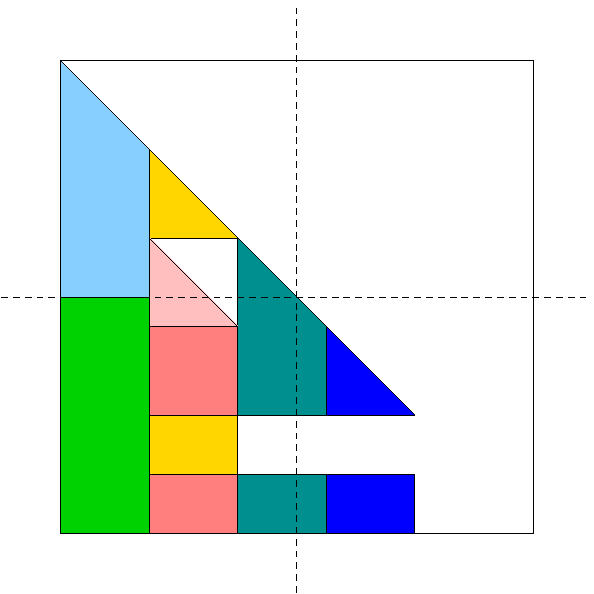
\includegraphics[width=\textwidth]{ARrec11}
        \end{center}
      \end{column}
    \end{columns}
  \end{block}
\end{frame}

%%%%%%%%%%%%%%%%%%%%%%%%%%%%%%%%%%%%%%%%%%%%%%%%%%%%%%%%%%%%%%%  
\begin{frame}[fragile]
\frametitle{LAPACK vs FFPACK modulo $8\,388\,593$}

{\footnotesize
  \begin{center}
\begin{tabular}{rrrrr}
\toprule
& \multicolumn{2}{c}{LAPACK}&\multicolumn{2}{c}{FFPACK}\\
$n$ & dgetrf (LU)  & dsytrf (LDLT) & fgetrf (LU)& fsytrf (LDLT)\\
\midrule
5000 &  2.01s & 1.60s  & 3.90s& \alert{1.59s} \\
10000 &  14.95s & 11.98s  & 24.12s& \alert{10.90s} \\
\bottomrule
\end{tabular}
\end{center}
}
%\vspace{-5pt}
%\hspace{-20pt}
%\begin{minipage}{\textwidth}
\scriptsize
%\onslide+<2>
\begin{center}
  \begin{gnuplot}[terminal=cairolatex,terminaloptions={font ",10" linewidth 2}]
  set style line 3 pt 3 pi 50 lw 4 lt rgb "blue"
  set title 'Full rank, 1-core Intel Haswell i5-4690, \symbol{64}3.5GHz' offset 0,-0.75
  set ylabel 'Effective Gfops' offset 1,0
  set xlabel 'matrix dimension' offset 0,0.1
  set xtics rotate by 30 offset -2,-0.75
  set y2tics autofreq 
  set autoscale y2fixmin
  set autoscale y2fixmax  
  set size 0.8,0.75
  set key bottom right Left reverse
  plot [1:10000] [1:45] \
  "data_gflops.txt" using 1:2 title "LAPACK dgetrf" with lines lw 4 lc 1, \ 
  "data_gflops.txt" using 1:3 title "LAPACK dsytrf" with lines lw 4 lc 2, \
  "data_gflops.txt" using 1:6 title "FFPACK fgetrf" with lines lw 4 lc 4, \
  "data_gflops.txt" using 1:7 title "FFPACK fsytrf" with lines ls 3
\end{gnuplot}
\end{center}
%\end{minipage}
\end{frame}
%%%%%%%%%%%%%%%%%%%%%%%%%%%%%%%%%%%%%%%
\begin{frame}
  \frametitle{Quasiseparable matrices }
  \begin{center}
    \textit{Matrices with low off-diagonal rank}
  \end{center}

  \begin{block}
    {[ISSAC'16, JSC'18] New compact representation and algorithms}
  \begin{columns}
    \begin{column}{.65\textwidth}
    \begin{itemize}
    \item Connection with rank profile matrix
    \item Matches the best space complexities: $O(ns)$
    \item Reduction to matrix multiplication: $O(ns^{\omega-1})$ for products
    \item Flat representation (non hierarchical)
    \end{itemize}
    \uncover<2->{
      \begin{description}
      \item[Follow-up:] on-going collaboration with numerical HPC experts:
        \begin{itemize}
        \item S. Chandrasekaran (UCSB)
        \item T. Mary (U. Manchester, \texttt{Mumps})
        \end{itemize}
      \end{description}
      }
    \end{column}
    \begin{column}{.3\textwidth}
      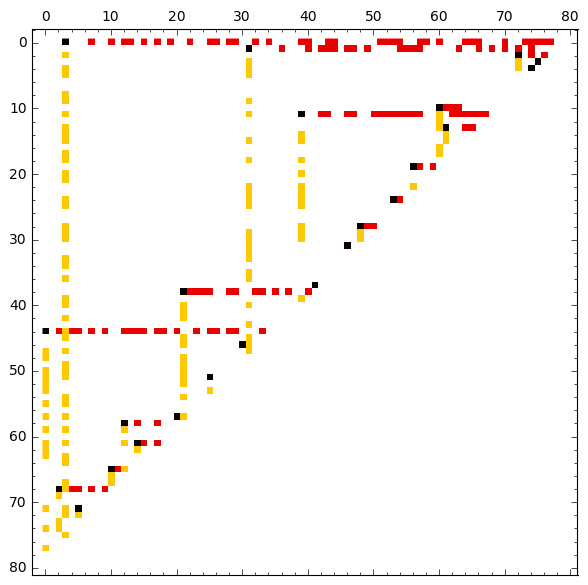
\includegraphics[width=\textwidth]{Bruhat}
    \end{column}
  \end{columns}
  \end{block}

\end{frame}


%%%%%%%%%%%%%%%%%%%%%%%%%%%%%%%%%%%%%%%
\begin{frame}
  \frametitle{Outsourced computing security}

  \begin{block}{Exploratory aspect: Computation over the Cloud}
    \begin{description}
    \item[Outsourcing computation on the cloud:]\ 
      \begin{itemize}
      \item trusted lightweitht client computer
      \item untrusted powerful cloud server
      \end{itemize}
      $\Rightarrow$ need for certification protocols
    \item[Multiparty computation:] \
      \begin{itemize}
      \item each player contribute with a share of the Input
      \item shares must remain private
      \end{itemize}
    \end{description}
\end{block}
  \begin{block}<2->
      {Contribution}
      \begin{description}
        \item[ISSAC'17:] Linear time certificates for LU, Det., Rank Profile  matrix, etc
        \item[In submission:] Secure multiparty Strassen's algorithm
      \end{description}
  \end{block}

\end{frame}
%%%%%%%%%%%%%%%%%%%%%%%%%%%%%%%%%%%%%%%
%%%%%%%%%%%%%%%%%%%%%%%%%%%%%%%%%%%%%%%%%%%%%%%%%%%%%%%%
\begin{frame}{Software releases and integration}
    \begin{block} {LinBox ecosystem}
      \begin{description}
        \item[\texttt{givaro}:] field/ring arithmetic
          \hfill{\uncover<2->{\alert{4 releases}}}
        \item[\texttt{fflas-ffpack}:] dense linear algebra over finite field \hfill{\uncover<2->{\alert{6 releases}}}
        \item[\texttt{LinBox}:] exact linear algebra \hfill{\uncover<2->{\alert{6 releases}}}
      \end{description}
      Tightly integrated  in \texttt{SageMath} \hfill{\uncover<2->{\alert{13 tickets}}}
    \end{block}

    \begin{block}<3-> {Featuring}
      \begin{itemize}
      \item Full functional implementations of new algorithmic contributions
      \item Improved vectorization and parallel routines
      \item Drastic improvement of reliability (continuous integration,
        test-suite coverage, randomized certificates, etc)
      \end{itemize}
    \end{block}
\end{frame}
%%%%%%%%%%%%%%%%%%%%%%%%%%%%%%%%%%%%%%%
%%%%%%%%%%%%%%%%%%%%%%%%%%%%%%%%%%%%%%%
\subsection{D5.11: Refactor and optimize Sage's Combinatorics}
\begin{frame}
  \frametitle{Task 5.6: HPC infrastructure for Combinatorics}

  \begin{center}
    {\bf \large
      Perform a Map/Reduce on huge recursive datasets.
    }
  \end{center}

  \begin{block}{Large range of intensive applications in combinatorics}
    Given a set $S$ of combinatorial objects we want to
    \begin{itemize}
    \item test conjectures: \textit{e.g.} find an element of $S$ satisfying a certain
      property
    \item count or list the elements of $S$ having this property
    \end{itemize}
  \end{block}

  \begin{block}{Specificities of combinatorics}
  Typically
    \begin{itemize}
    \item \textbf{huge}: $S$ does not fit in memory
    \item \textbf{embarassingly parallel}: $S = S_1 \cup \ldots \cup S_k$
    \item \textbf{unbalanced}: $S_i$ sizes are highly unbalanced
    \end{itemize}
  \end{block}
\end{frame}
%%%%%%%%%%%%%%%%%%%%%%%%%%%%%%%%%%%%%%%
\begin{frame}
  \frametitle{D5.11: Refactor and optimise the existing combinatorics Sage code using the new developed Pythran and Cython features.}

  \begin{enumerate}
  \item Problem examples
    \begin{enumerate}
    \item integer vectors and polytopes
    \item numerical semigroups
    \end{enumerate}
  \item Algorithmic innovations and experimentations:
    \begin{enumerate}
    \item map-reduce with \emph{work-stealing} strategy
    \item SIMD instructions for small combinatorial objects
    \item Python/Cython/Pythran
    \end{enumerate}
  \item Software releases and integration:
    \begin{enumerate}
    \item \texttt{SageMath} integration
    \item C/C++ libraries: \texttt{HPCombi}, \texttt{e-antic}
    \item Python library: \texttt{pplpy}
    \end{enumerate}
  \end{enumerate}

\end{frame}


\begin{frame}
  \frametitle{Example 1: integer vectors and polytopes}

\end{frame}


\begin{frame}
  \frametitle{Example 2: numerical semigroup}
\end{frame}

\begin{frame}
  \frametitle{Job-stealing map-reduce}
\end{frame}

\begin{frame}
  \frametitle{SIMD instructions for small combinatorial objects}
\end{frame}

\begin{frame}
  \frametitle{Python, Cython, Pythran and SIMD code}

\begin{center}
%  \begin{gnuplot}[terminal=cairolatex,terminaloptions={font ",10" linewidth 2}]
%  set style line 3 pt 3 pi 50 lw 4 lt rgb "blue"
%  set title 'Counting descents in permutations'
%  set ylabel 'log time' offset 1,0
%  set xlabel 'n' offset 0,0.1
%  set xtics rotate by 30 offset -2,-0.75
%  set y2tics autofreq 
%  set autoscale y2fixmin
%  set autoscale y2fixmax  
%  set size 0.8,0.75
%  set key bottom right Left reverse
%  plot [8:13] [1:500] "data_perms.txt" using 1:4 
%  "data_perms.txt" using 1:3 title "Cython list" with lines lw 3 lc 2, \
%  "data_perms.txt" using 1:4 title "Cython array" with lines ls 3
%  \end{gnuplot}
\end{center}

\end{frame}


\begin{frame}{Software releases and integration}
    \begin{block} {Libraries releases and integration}
      \begin{description}
        \item[\texttt{SageMath}:] \hfill{\uncover<2->{\alert{5 tickets}}}
        \item[\texttt{HPCombi}:] C++ library for small combinatorial objects
	using SIMD instructions and fine grained parallelization (Cilk)
	\item[\texttt{e-antic}]: C/C++ library for (arbitrary precision) embedded
	number field computations
	\item[\texttt{pplpy}:] Python library interface to PPL library on Polytope
	\hfill{\uncover<2->{\alert{6 releases}}}
      \end{description}
    \end{block}

    \begin{block}<3-> {Featuring}
      \begin{itemize}
      \item SIMD instructions for combinatorial enumeration
      \item Fast code inside SageMath
      \end{itemize}
    \end{block}

\end{frame}

%%%%%%%%%%%%%%%%%%%%%%%%%%%%%%%%%%%%%%%
%% \subsection{Task 5.7: Pythran}
%% \begin{frame}
%%   \frametitle{Task 5.7: Pythran}
%%   \begin{center}
%%     {\Large \textbf{Pythran}: a Python to C compiler}
%%   \end{center}
%%   \begin{columns}
%%     \begin{column}
%%       {.48\textwidth }
%%           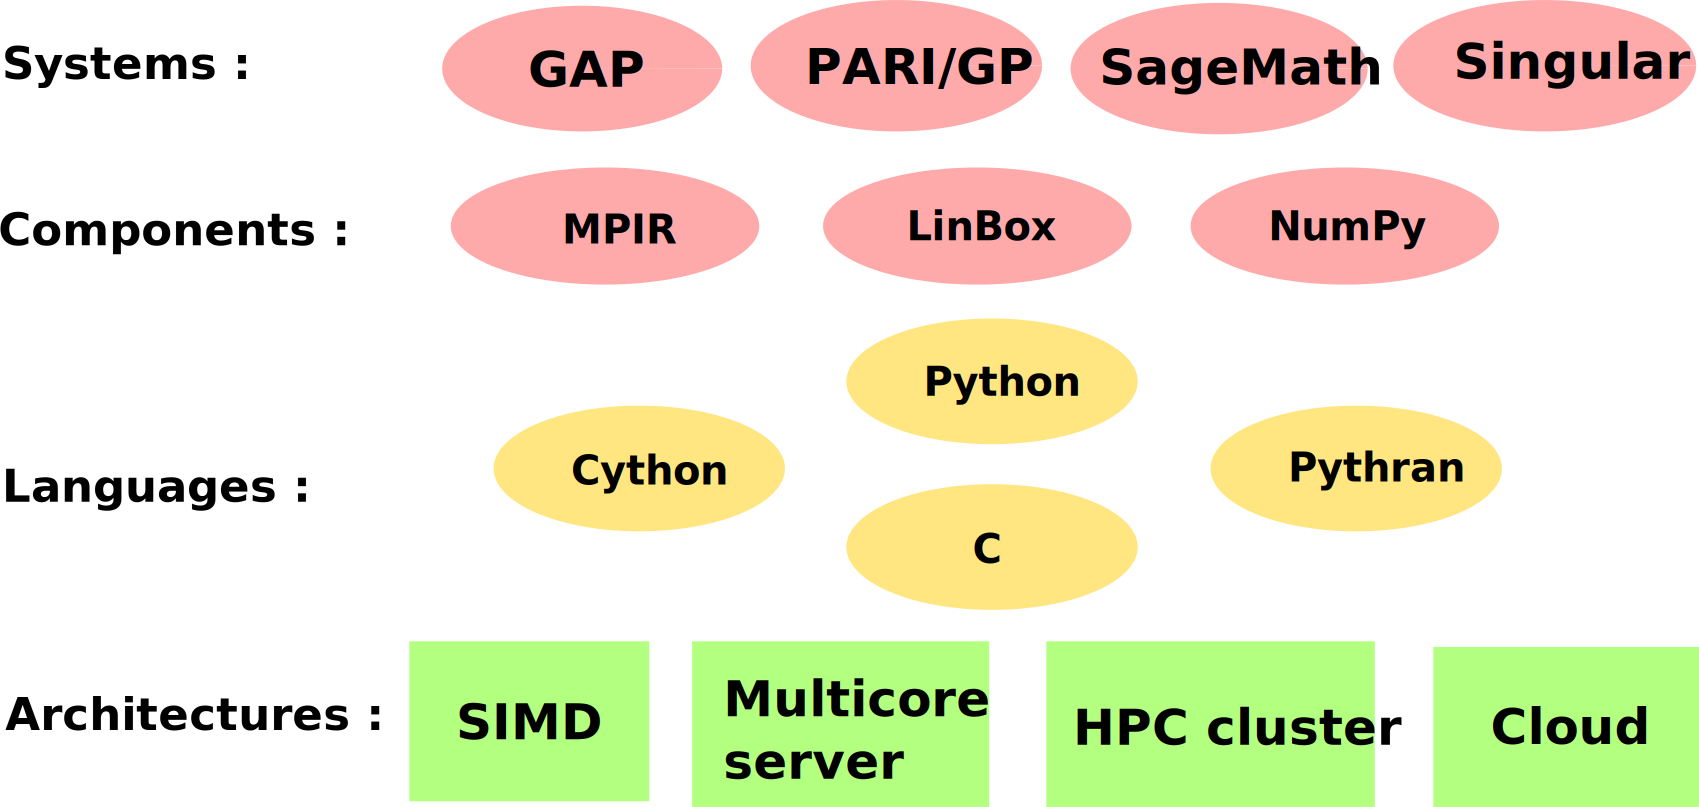
\includegraphics[width=\textwidth]{software_stack}
%%     \end{column}
%%     \begin{column}
%%       {.48\textwidth }
%%   \begin{itemize}
%%   \item High level VRE rely on the Python language
%%   \item High performance is achieved mostly by the C language\pause
%%   \item Python to C compilers: 
%%     \begin{itemize}
%%     \item Cython: general purpose
%%     \item Pythran: narrower scope, better at optimizing Numpy code (Linear
%%       algebra)
%%     \end{itemize}
%%   \end{itemize}
%%     \end{column}
%%   \end{columns}
%% \pause
%%   \begin{center}
%%     \textbf{Goal: Implement the convergence}

%%     \begin{description}
%%       \item[D5.4] Improve Pythran typing system
%%       \item[D5.2] Make Cython use Pythran backend to optimize Numpy code
%%     \end{description}
%%   \end{center}
  
%% \end{frame}
%%%%%%%%%%%%%%%%%%%%%%%%%%%%%%%%%%%%%%%
%% \begin{frame}[fragile]
%%   \frametitle{D5.2: Make Cython use Pythran backend for NumPy code}

%%   \begin{center}
%%     \includegraphics[width=.65\textwidth]{float_graph}\\
%%   \end{center}
%%   \begin{lstlisting}
%% import numpy
%% cimport numpy
%% def float_comp (numpy.ndarray[numpy.float_t, ndim=1] a,
%%                  numpy.ndarray[numpy.float_t, ndim=1] b):
%%      return numpy.sqrt(numpy.sqrt(a*a+b*b))
%% \end{lstlisting}

%% \end{frame}
%% %%%%%%%%%%%%%%%%%%%%%%%%%%%%%%%%%%%%%%%%%%%%%%%%%%%%%%%%%%%%%%%%%%
%% \begin{frame}[fragile]
%%   \frametitle{D5.2: Make Cython use Pythran backend for NumPy code}

%%   \begin{center}
%%     \includegraphics[width=.65\textwidth]{harris_graph}
%%   \end{center}
  
%%   \begin{lstlisting}[basicstyle=\tiny]
%% def harris(numpy.ndarray[numpy.float_t, ndim=2] I):
%%   cdef int m = I.shape[0]
%%   cdef int n = I.shape[1]
%%   cdef numpy.ndarray[numpy.float_t,ndim=2] dx = (I[1:,:] - I[:m-1,:])[:,1:]
%%   cdef numpy.ndarray[numpy.float_t,ndim=2] dy = (I[:,1:] - I[:,:n-1])[1:,:]
%%   cdef numpy.ndarray[numpy.float_t, ndim=2] A = dx * dx
%%   cdef numpy.ndarray[numpy.float_t, ndim=2] B = dy * dy
%%   cdef numpy.ndarray[numpy.float_t, ndim=2] C = dx * dy
%%   cdef numpy.ndarray[numpy.float_t, ndim=2] tr = A + B
%%   cdef numpy.ndarray[numpy.float_t, ndim=2] det = A * B - C * C
%%   return det - tr * tr
%% \end{lstlisting}

%% \end{frame}

%%%%%%%%%%%%%%%%%%%%%%%%%%%%%%%%%%%%%%%
%% \begin{frame}
%%       \frametitle{D5.4: Improve Pythran typing system}
%% \end{frame}

%%%%%%%%%%%%%%%%%%%%%%%%%%%%%%%%%%%%%%%
%%%%%%%%%%%%%%%%%%%%%%%%%%%%%%%%%%%%%%%
\section{Progress report on other deliverables}
%%%%%%%%%%%%%%%%%%%%%%%%%%%%%%%%%%%%%%%
\subsection{T5.1: Pari}
\begin{frame}
  \frametitle{T5.1: Pari}
  \begin{block} {D5.16: Pari Suite release, fully supporting parallelization}
    \begin{itemize}
    \item D5.10 (merged in D5.16):\\ Generic parallelization engine is now mature
      (released since nov.2016). Support POSIX-threads and MPI.
    \item Current work: applying it throughout the library
      \begin{itemize}
      \item Chinese remaindering
      \item Rational linear algebra
      \item Discrete logarithm
      \item Resultants
      \item APRCL primality testing
      \end{itemize}
      
      
    \end{itemize}
  \end{block}
\end{frame}

%%%%%%%%%%%%%%%%%%%%%%%%%%%%%%%%%%%%%%%
\subsection{T5.2: GAP}
\begin{frame}
  \frametitle{T5.2: GAP}
  \begin{block} {D5.15: Final report of GAP development}
    \begin{itemize}
    \item 8 releases were cut integrating contributions of D3.11 and D5.15
    \item Towards an integration of HPC-GAP: main release GAP-4.9
      \begin{itemize}
      \item Build system refactoring
      \item Ability to compile in HPC-GAP compatibility mode
      \end{itemize}
    \item Work in progress:
      \begin{itemize}
      \item  Multithreaded linear algebra: at the level of the \texttt{Meataxe} library
      \item Introspection functionalities: on-the-fly optimisaiton decision
      \end{itemize}
    \end{itemize}
  \end{block}
\end{frame}

%%%%%%%%%%%%%%%%%%%%%%%%%%%%%%%%%%%%%%%
\subsection{T5.3: LinBox}
\begin{frame}
  \frametitle{T5.3 LinBox}

  \begin{block} {D5.14: Distributed exact linear system solving}
{
    \only<1,2>{
      \begin{itemize}
        \item 2 full time engineers
        \item Comm. and serialization layer done
        \item Prototype MPI parallelization of Chinese remainder based solver.
      \end{itemize}
    }
    \only<3->{
      \begin{description}
      \item[Roadmap:] \
        \begin{itemize}
        \item Major refactorization of LinBox solver code under way
        \item Parallelization of Dixon-lifting solver
        \item Hybrid combination of CRT+Dixon.
        \item Hyrbid OpenMP-MPI implementation
        \end{itemize}   
      \end{description}
        \vspace{-1.4em}
    }
    \begin{columns}
      \begin{column} {.5\textwidth}
        \begin{center}
          \uncover<2->{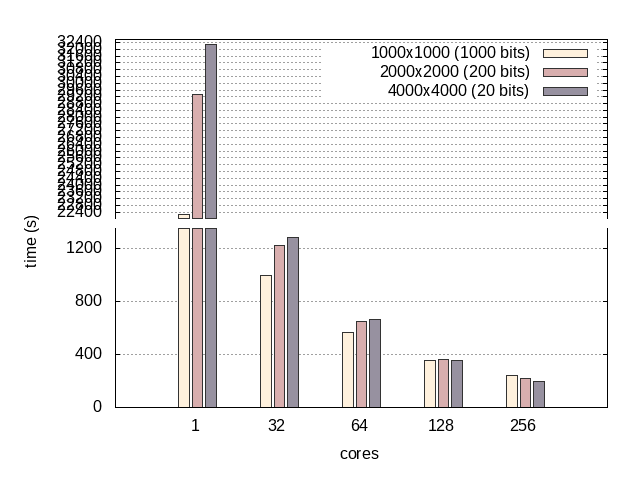
\includegraphics[width=\textwidth]{nodes_histogram}}
      \end{center}
      \end{column}
      \begin{column} {.45\textwidth}
        \begin{center}
          \uncover<2->{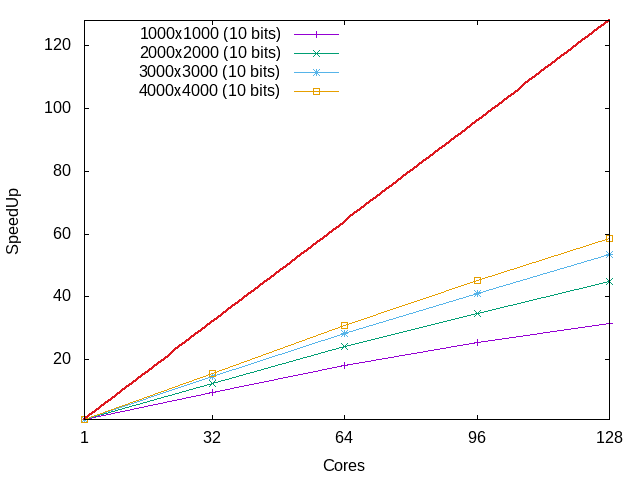
\includegraphics[width=\textwidth]{nodes_SPEEDUP}}
        \end{center}
      \end{column}
    \end{columns}
}
  \end{block}
\end{frame}
%%%%%%%%%%%%%%%%%%%%%%%%%%%%%%%%%%%%%%%%%%%%%%%%%%%%
\subsection{T5.4: Singular}
\begin{frame}
  \frametitle{T5.4 Singular}
  \begin{block}
    {D5.13: Paralell sparse polynomial multiplication}
    
    \texttt{FLINT} now support fast sparse multivariate polynomials:
    \begin{itemize}
    \item addition, subtraction, multiplication,
    \item division, division with remainder, GCD
    \item evaluation (and partial evaluation), composition
    \end{itemize}

\uncover<2->{  \textbf{Parallelization of the (sparse) multiplication}
    \begin{columns}
      \begin{column}{.38\textwidth}
        {\footnotesize
          %% \begin{equation*}
          %%   (1 + x + y + 2z^2 + 3t^3 + 5u^5)^{21}*(1 + u + t + 2z^2 + 3y^3 + 5x^5)^{21}
          %% \end{equation*}
%          \begin{center}
            \begin{tabular}{lcccccccc}
               \toprule
               threads & time (ms) & speedup\\ \midrule
               1 & 148661 & 1.0x\\
               2 & 76881 & 1.9x\\ 
               3 & 54798 & 2.7x\\ 
               4 & 42855 & 3.4x\\ 
               5 & 37017 & 4.0x\\ 
               6 & 30892 & 4.8x\\ 
               7 & 28365 & 5.2x\\ 
               8 & 28048 & 5.3x\\
               \bottomrule
            \end{tabular}
 %         \end{center}
        }
      \end{column}
      \begin{column}{.6\textwidth}
        \uncover<3->{
          \begin{itemize}
        \item Planned improvements to the memory manager $\Rightarrow$ closer to linear scaling 
        \item Parallel division and GCD implementations are in progress.
        \item Integration into Factory/Singular remains to be done
          \end{itemize}
          }
      \end{column}
    \end{columns}
    }
   \end{block}

 \end{frame}

%% \begin{frame}
%%   \frametitle{Root clustering}
    
%%     \begin{block}{Root clustering}
%% \begin{itemize}
%%  \item Remi Imbach has implemented the new parallel root clustering algorithm of Sagraloff-Yap
%%  \item Remi will return to Kaiserslautern (from New York visiting Chee Yap) to integrate the new code in Singular
%%  \item All deliverables for Kaiserslautern are on track
%%  \end{itemize}

%%  \end{block}
%%  \end{frame}

%%%%%%%%%%%%%%%%%%%%%%%%%%%%%%%%%%%%%%%
\section{Workpackage management}

\subsection{Milestone M8}
\begin{frame}[fragile]
  \frametitle{Milestone M8: Seamless use of parallel computing architecture in the VRE (proof of concept)}

{\footnotesize  \textit{Astrid wants to run compute intensive routines involving both dense linear algebra and combinatorics. She has access through a JupyterHub-based VRE to a high end multi-core machine which includes a vanilla SAGE installation.
She automatically benefits from the HPC features of the underlying specialized libraries (LinBox, ...). This is a proof of concept of the overall framework to integrate the HPC advances of specialized libraries into a general purpose VRE. It will prepare the final integration of a broader set of such parallel features for the end of the project}


\begin{verbatim}
sage: a=random_matrix(GF(11),8000,8000)
sage: time b=a*a
CPU times: user 1min 23s, sys: 1min 14s, total: 2min 37s
Wall time: 7.14 s
\end{verbatim}
}

\end{frame}
%%%%%%%%%%%%%%%%%%%%%%%%%%%%%%%%%%%%%%%%%%%%%%%%%
\subsection{Strenghtening interactions with numerical HPC}
\begin{frame}
\frametitle{Addressing recommendations of review 1}
    \textbf{Recommendation 10:} \textit{Regarding WP5, \textbf{make contacts} with HPC community in order to ascertain current state-of-the-art. The work in this WP needs to be \textbf{nearer the leading edge}.}
    \begin{description}
    \item<2-> [Leading edge achievements in linear algebra] \
      {\small
      \begin{itemize}
      \item symmetric factorization outperforms LAPACK implementation
      \item new non-hierarchical generator for quasiseparable matrices
      \item large scale parallelization of rational linear solver
      \end{itemize}
      }
    \begin{columns}
      \begin{column} {.3\textwidth}
        \begin{center}
          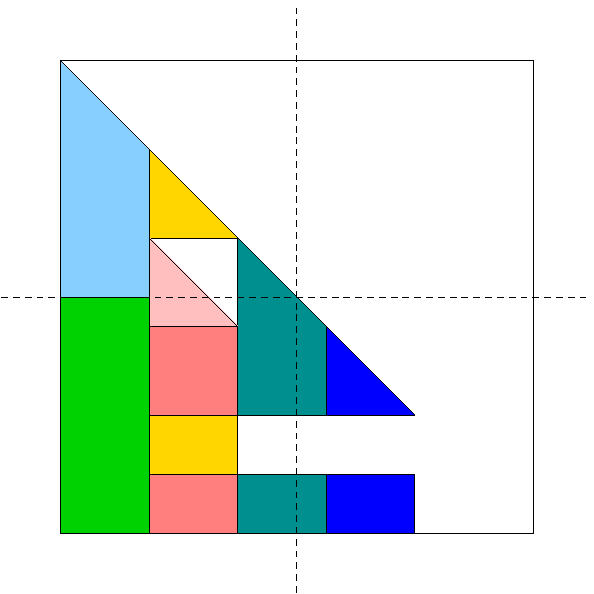
\includegraphics[width=.6\textwidth]{ARrec11}
      \end{center}
      \end{column}
      \begin{column} {.3\textwidth}
        \begin{center}
          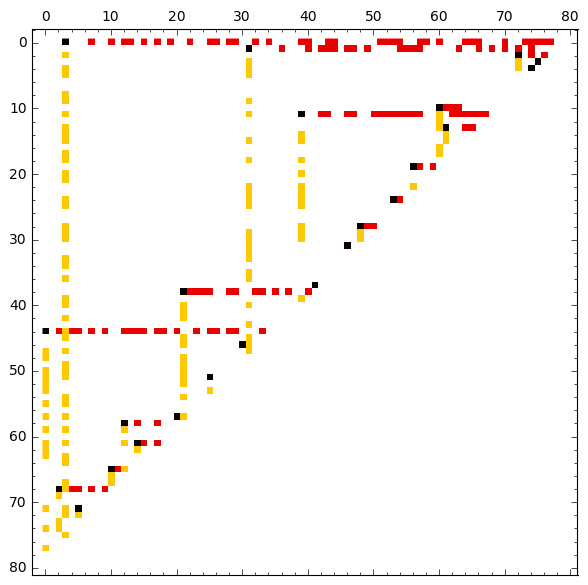
\includegraphics[width=.6\textwidth]{Bruhat}
        \end{center}
      \end{column}
      \begin{column} {.3\textwidth}
        \begin{center}
          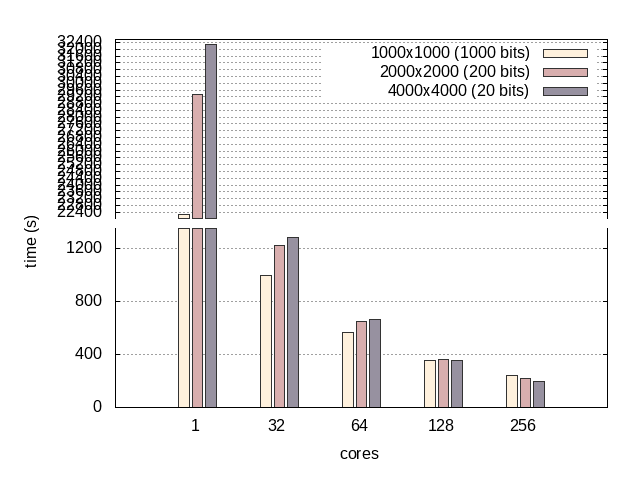
\includegraphics[width=.9\textwidth]{nodes_histogram}
        \end{center}
      \end{column}
    \end{columns}
\end{description}
\end{frame}

\begin{frame}
  \frametitle{Interaction with numerical HPC community}
  \begin{block}  {Existing connection}
    \begin{itemize}
    \item  dense linear algebra: numerical BLAS used for exact FFLAS for 17 years
    \item pointwise interactions with J Dongarra, L. Grigori, J-Y. L'Excellent,  etc
    \item publishing in major HPC venues:
      SIAM-PPSC, EuroPar, PMAA, ParCo
    \item Involvement in the french CNRS GDR-Calcul  working group (Sci Comp)
    \end{itemize}
  \end{block}
  \begin{block}<2->  {Recently established}
    \begin{itemize}
    \item with the \texttt{BLIS} group:
      \begin{itemize}
      \item SIMD vectorization bug report and user experience
      \item Implementation of Strassen's algorithm
      \end{itemize}
    \item on-going collaboration with T. Mary (\texttt{Mumps}) and
        S. Chandrasekaran (UCSB) on quasiseparable matrix algorithmic
    \end{itemize}
  \end{block}
\end{frame}
%%%%%%%%%%%%%%%%%%%%%%%%%%%%%%%%%%%%%%%
%%%%%%%%%%%%%%%%%%%%%%%%%%%%%%%%%%%%%%%
\end{document}
